\section*{Digital Timing}
Digital timing algorithm uses directly the digitized waveforms, performing a digital signal treatment similar to the analog one.
 
The CFD method works generating a bipolar signal from the original pulse and then computing its zero crossing as time reference. Lets name $W_t$ the digitized waveform with $t$ an integer number (sample number). The bipolar pulse $P_t$ is calculated as:
\begin{equation}
P_t=\chi W_t-W_{t-\delta},
\label{eq:bipolarCFD}
\end{equation}
where $\chi$ is a reduction fraction and $\delta$ an integer delay.  Fig.~\ref{Fig:DigitalCFD} shows the CFD method applied on a signal. 
\begin{figure}[h!]
	\centering
	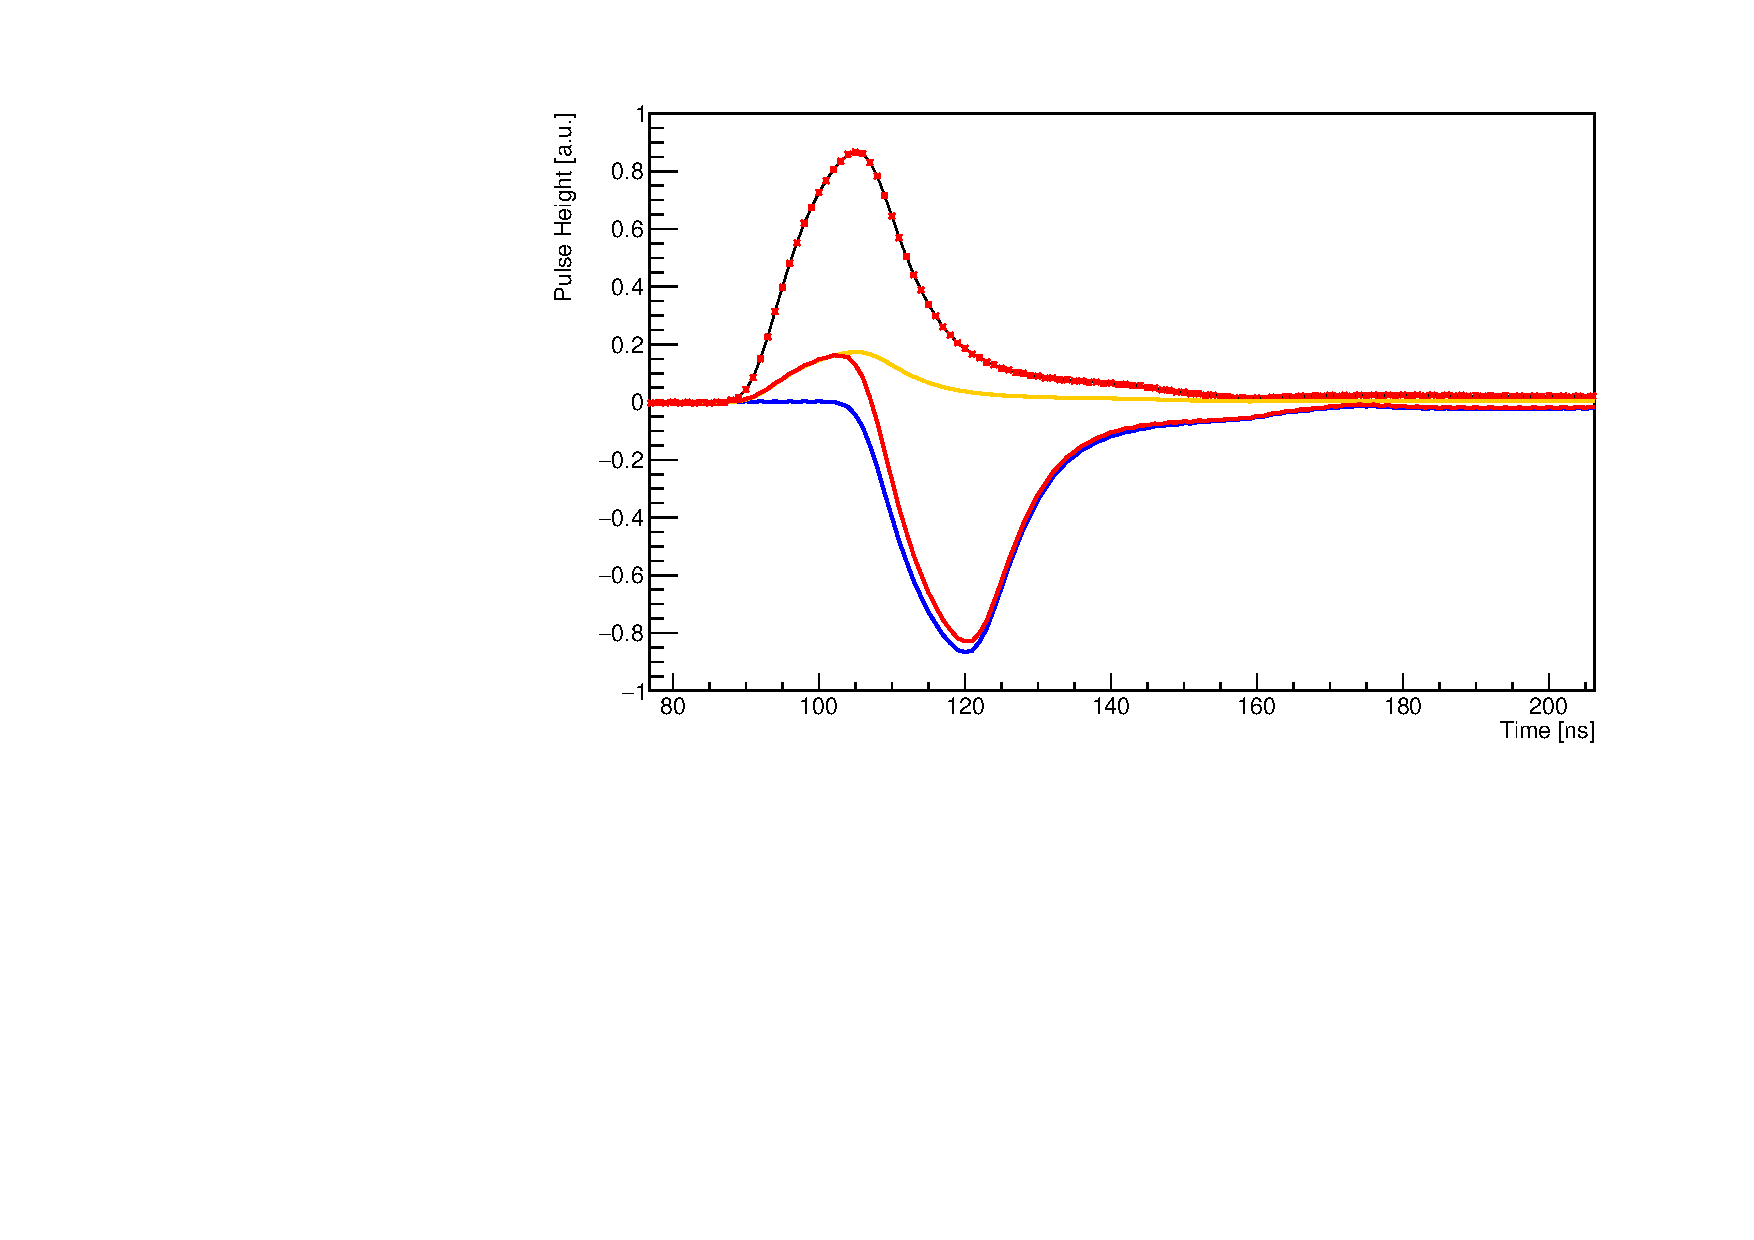
\includegraphics[width=\textwidth]{AverageCFD}
	\caption{Digital waveform obtained as an average of $10^4$ normalized signals. The Delayed and fractioned signals with their sum are represented too. }
	\label{Fig:DigitalCFD}
\end{figure}

\newpage
To increase the precision and reduce the dependence on the signal amplitude (time walk), the intersection with a zero crossing line is used. It is found by taking the samples above and below  it  and interpolating to find the time reference. 
A cubic spline interpolation with derivative bound continuity condition up to second order was chosen.
Lets consider the sample range $[t_{-1},t_{0}]$ with $t_{0}$ the first sampled point after the intersection and $t_{-1}$ the preceding one. The reconstructed pulse $f(t)$ inside the range is evaluated as follow:\\
\[\mathbf{f(t)=a (t-t_{-1})^3+b (t-t_{-1})^2+c (t-t_{-1})+d}\]
\[
\left\{
\begin{aligned}
a &=1/18 (P_{t_{-3}}-8 P_{t_{-2}}+19 P_{t_{-1}}-19 P_{t_{0}}+8 P_{t_{1}}-P_{t_{2}})\\
b &=1/30 (-4 P_{t_{-3}}+32 P_{t_{-2}}-58 P_{t_{-1}}+37 P_{t_{0}}-8 P_{t_{1}}+ P_{t_{2}})\\
c &=1/90 (7 P_{t_{-3}}-56 P_{t_{-2}}-11 P_{t_{-1}}+74 P_{t_{0}}-16 P_{t_{1}}+2 P_{t_{2}})\\
d &=P_{t_{-1}}
\end{aligned}
\right.
\]

Similarly to the analog timing, an optimization of the CFD parameters was necessary.  A first grid search was performed over several fractions and delays, selecting events inside a thin energy slice centered on the Compton edge.  Fig.~\ref{Fig:Surf28} shows the best parameters configuration with little delays and fractions. However these are not the right choice, with too low delay and fraction the bipolar signals formed would be to small and many events would be lost. This behavior is highlighted observing the density plot of the timing distribution integral inside the FWHM range shown in Fig.~\ref{Fig:Surf_int28}. 

\begin{figure}[H]
	\centering
	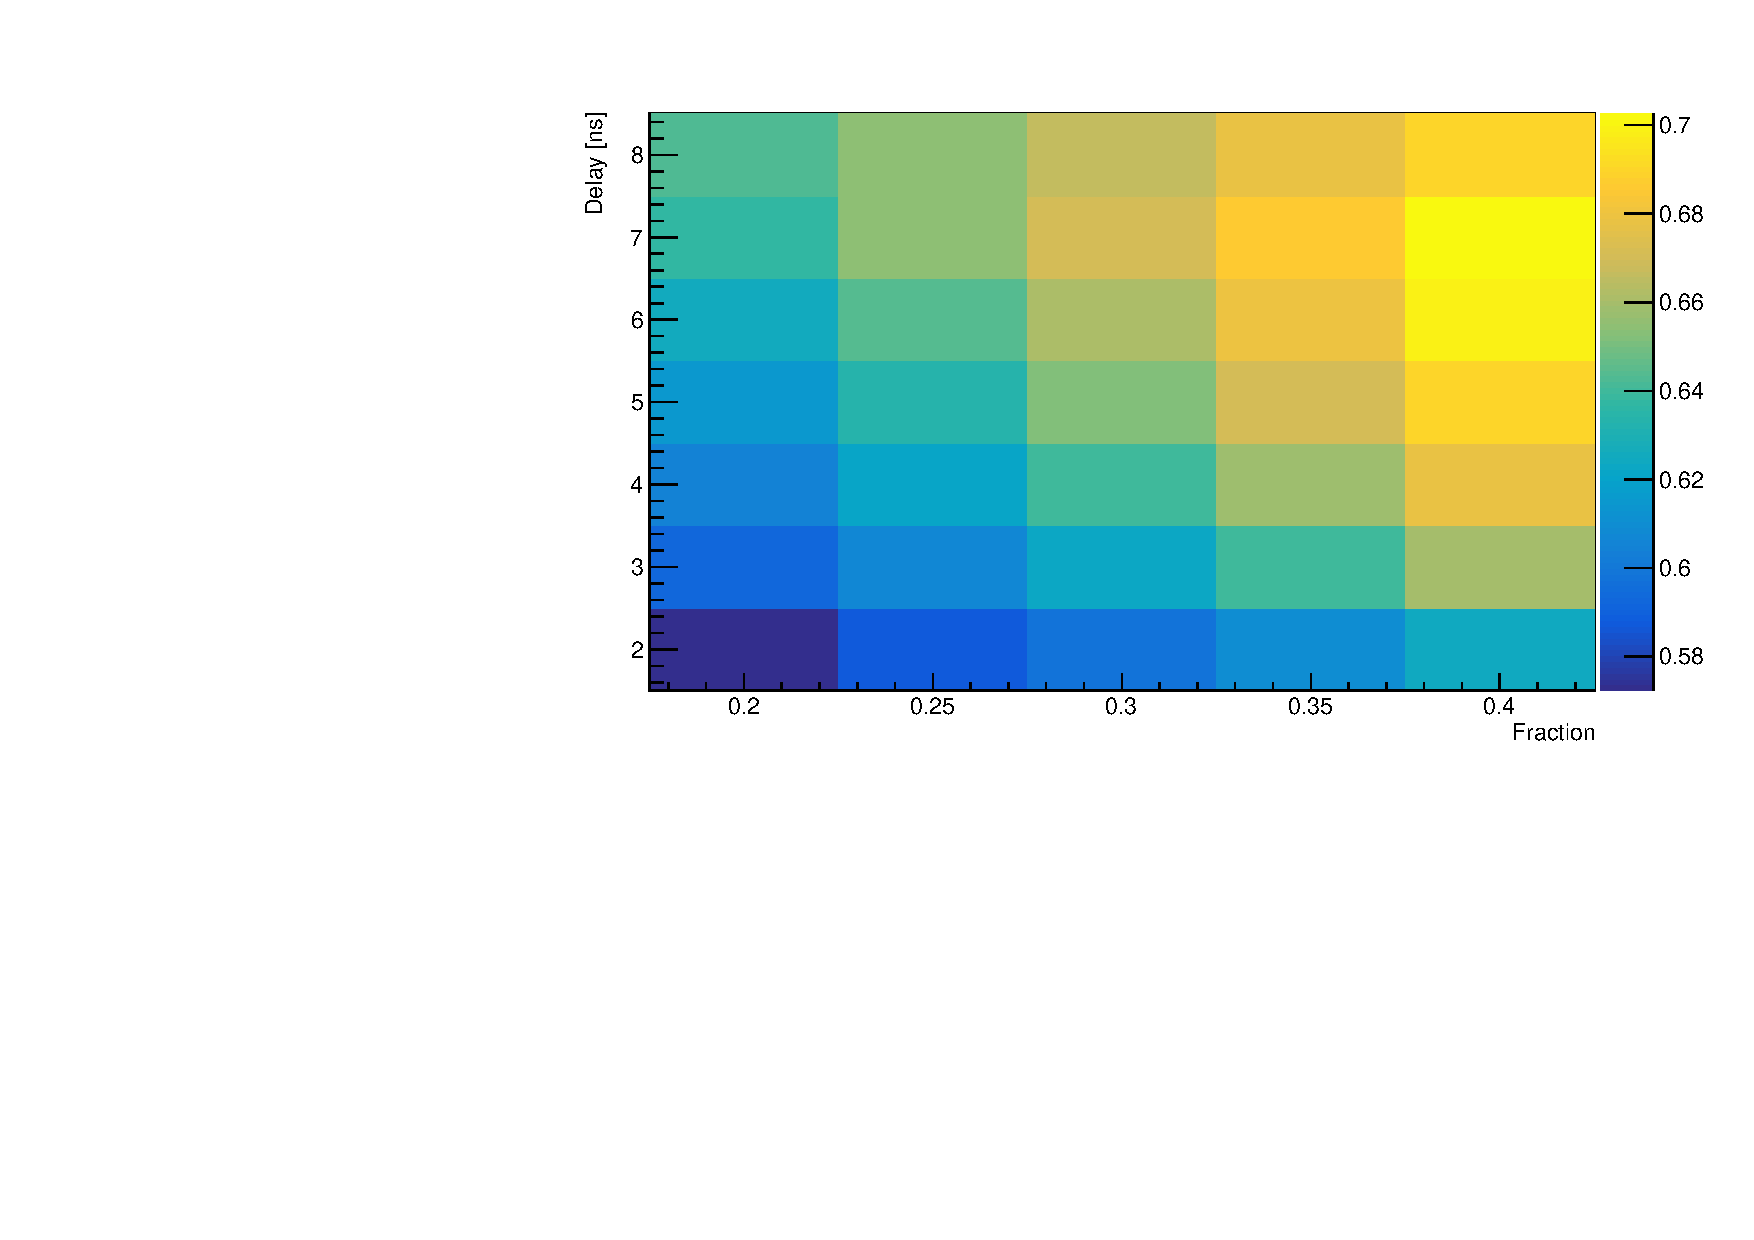
\includegraphics[width=\textwidth]{2_8surf}
	\caption{2-D density plot of digital timing distribution FWHM obtained with different delays and fractions.}
	\label{Fig:Surf28}
\end{figure}

\begin{figure}[H]
	\centering
	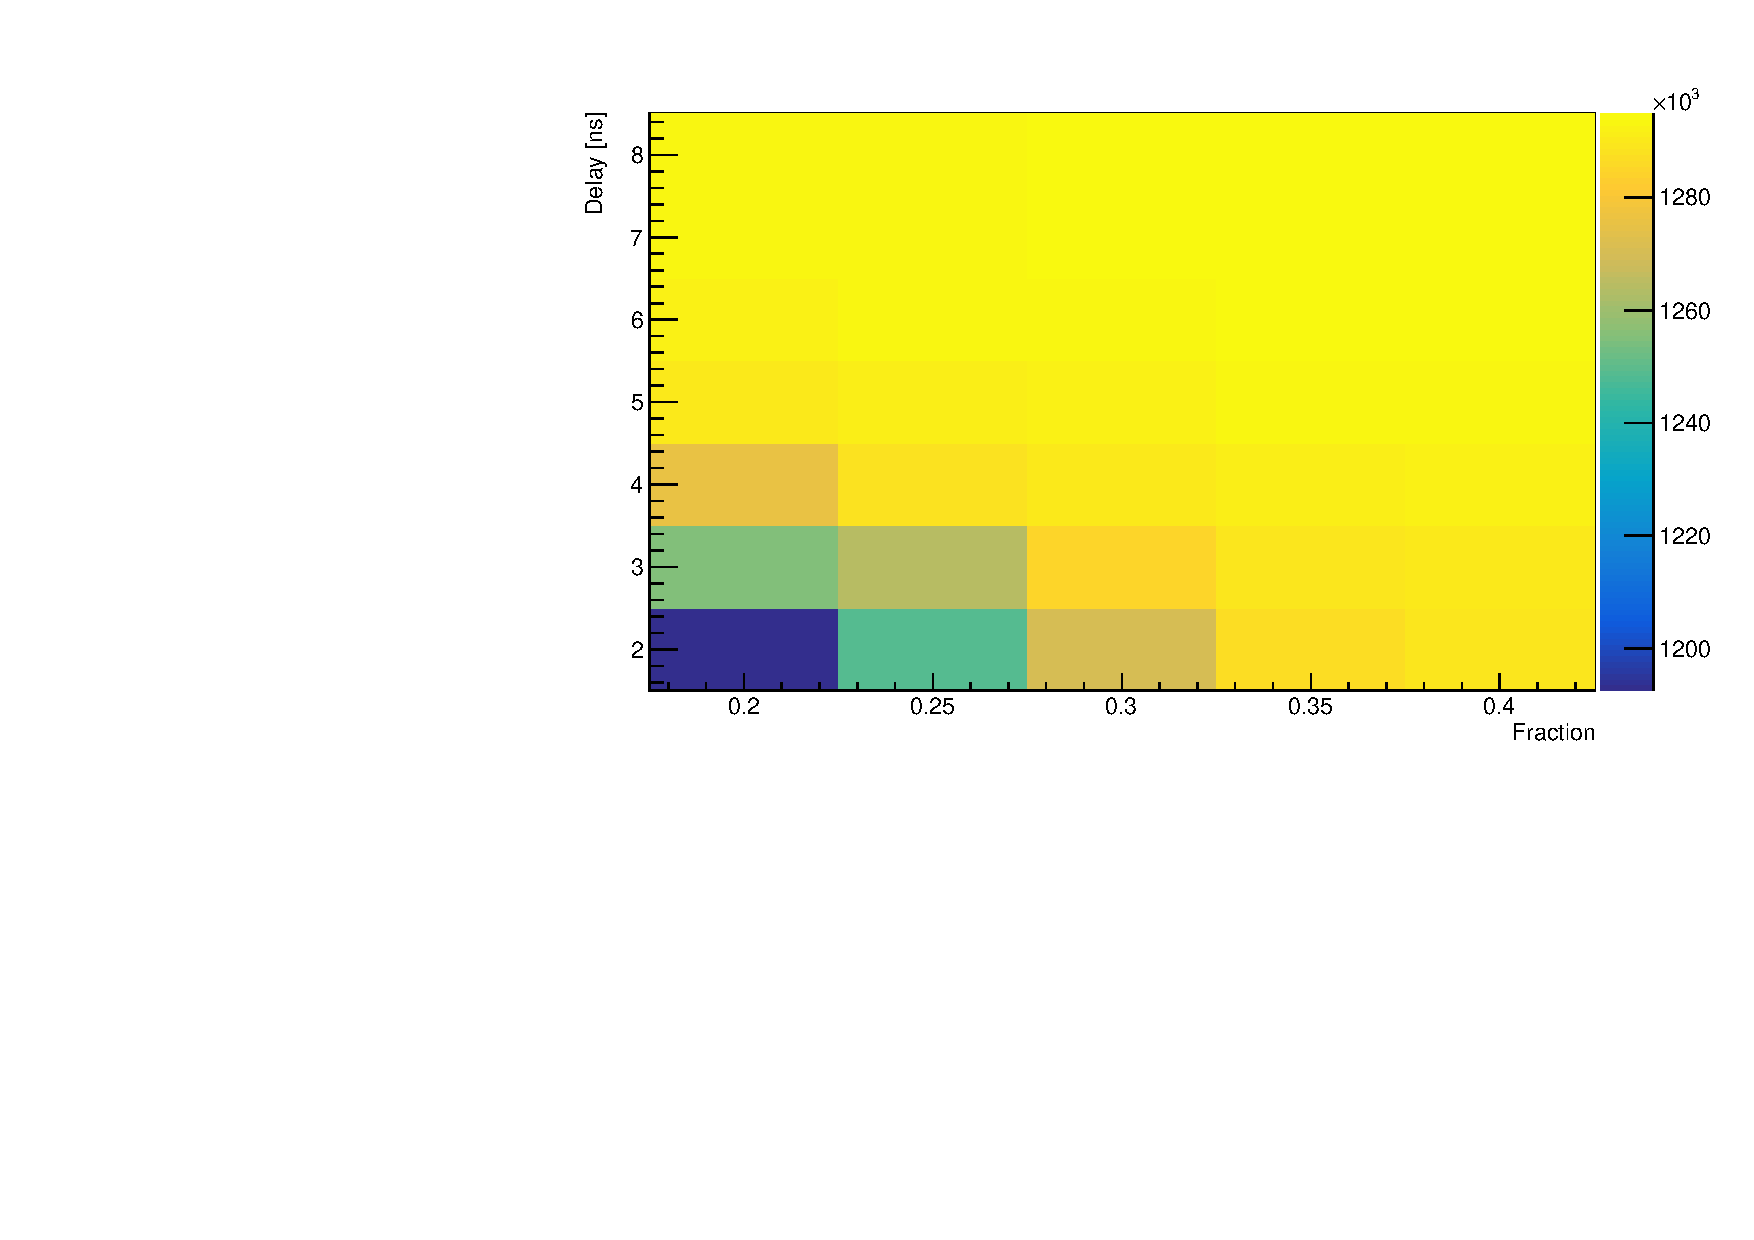
\includegraphics[width=\textwidth]{2_8int_surf}
	\caption{2-D density plot of timing distribution integral inside the FWHM range, with different delays and fractions.}
	\label{Fig:Surf_int28}
\end{figure}
 
 A new grid search was performed (see Fig.~\ref{Fig:fd_opt}) finding the best resolution with:
 \[
 \begin{aligned}
\text{Fraction} &=0.16\\
\text{Delay}  &= 11 \text{~ns}
 \end{aligned}
 \]
 
 \begin{figure}[H]
 	\centering
 	\subfloat[][\emph{Fraction}.]
 	{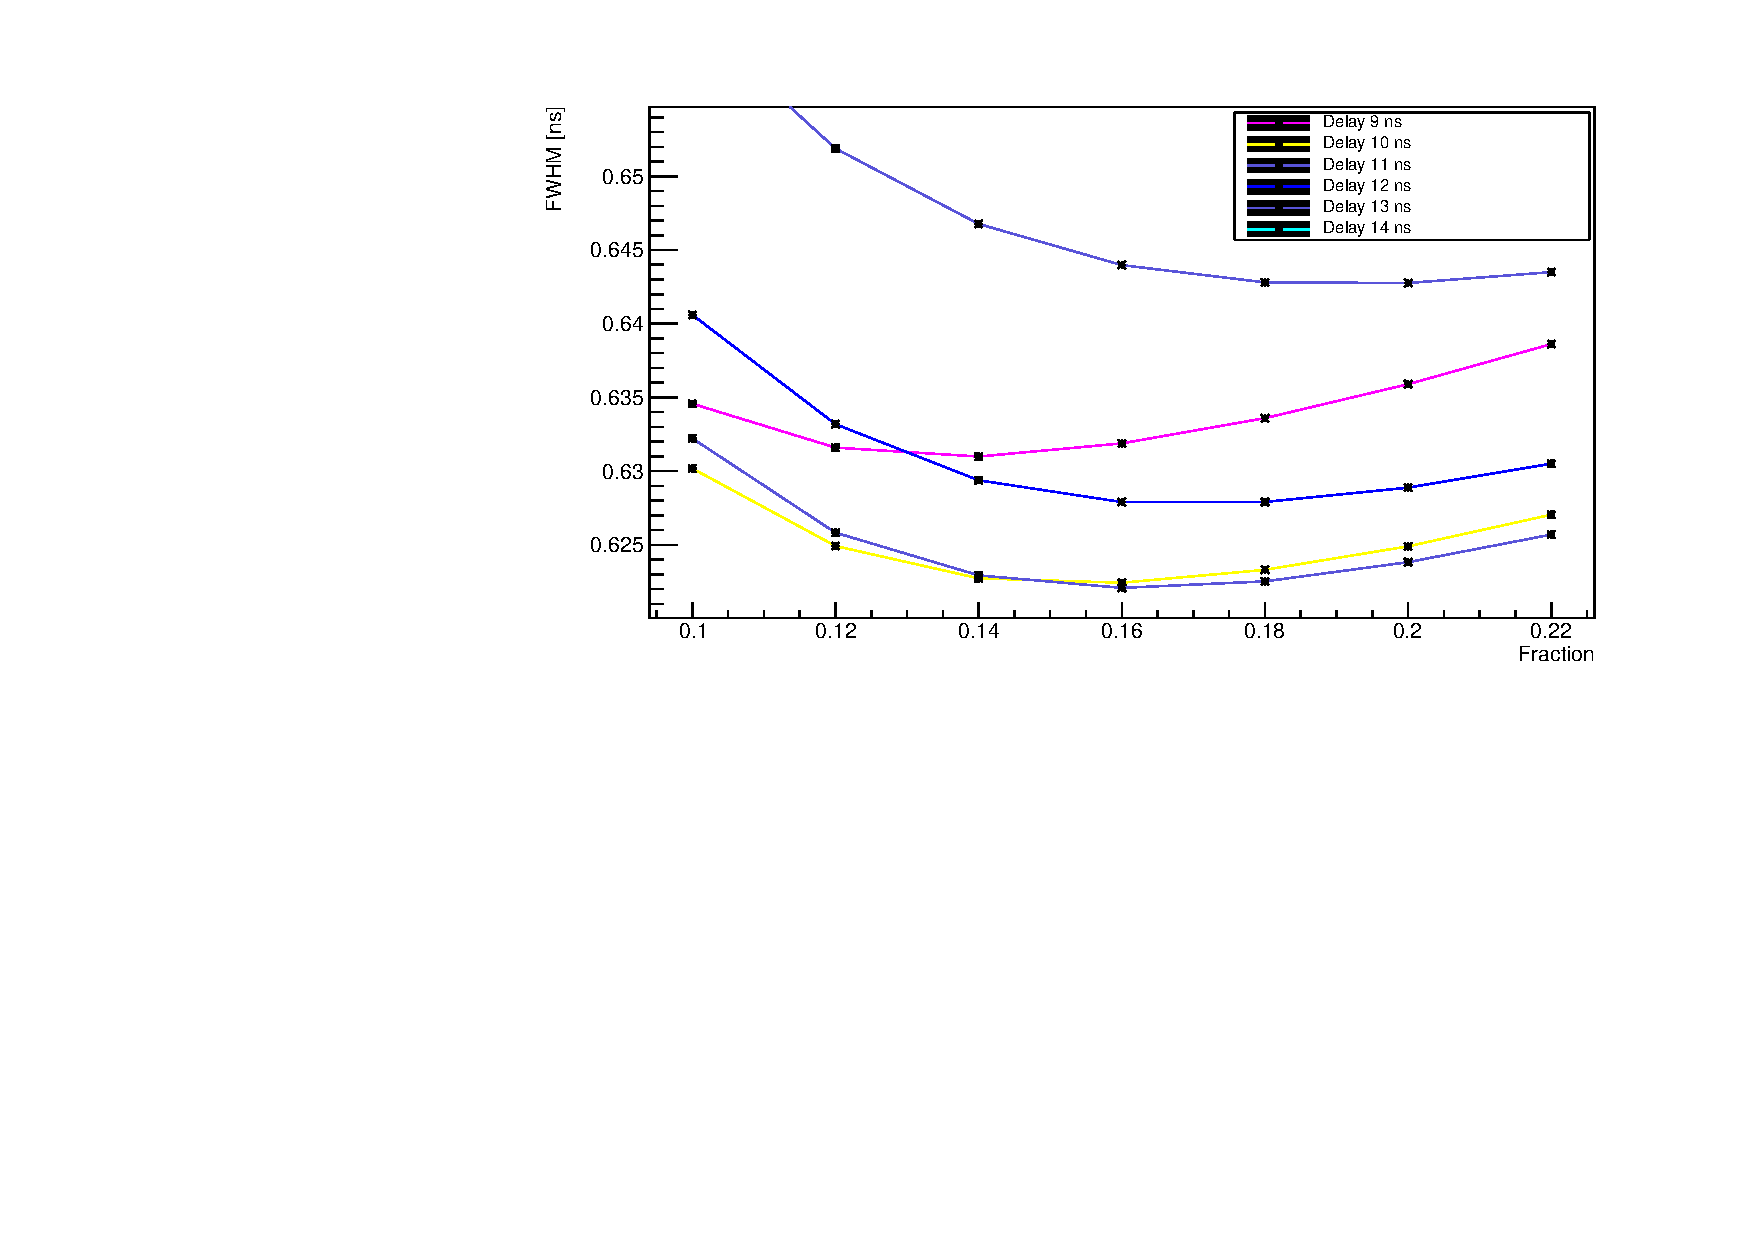
\includegraphics[width=.48\textwidth]{8_14_frac}} \quad
 	\subfloat[][\emph{Delay}.]
 	{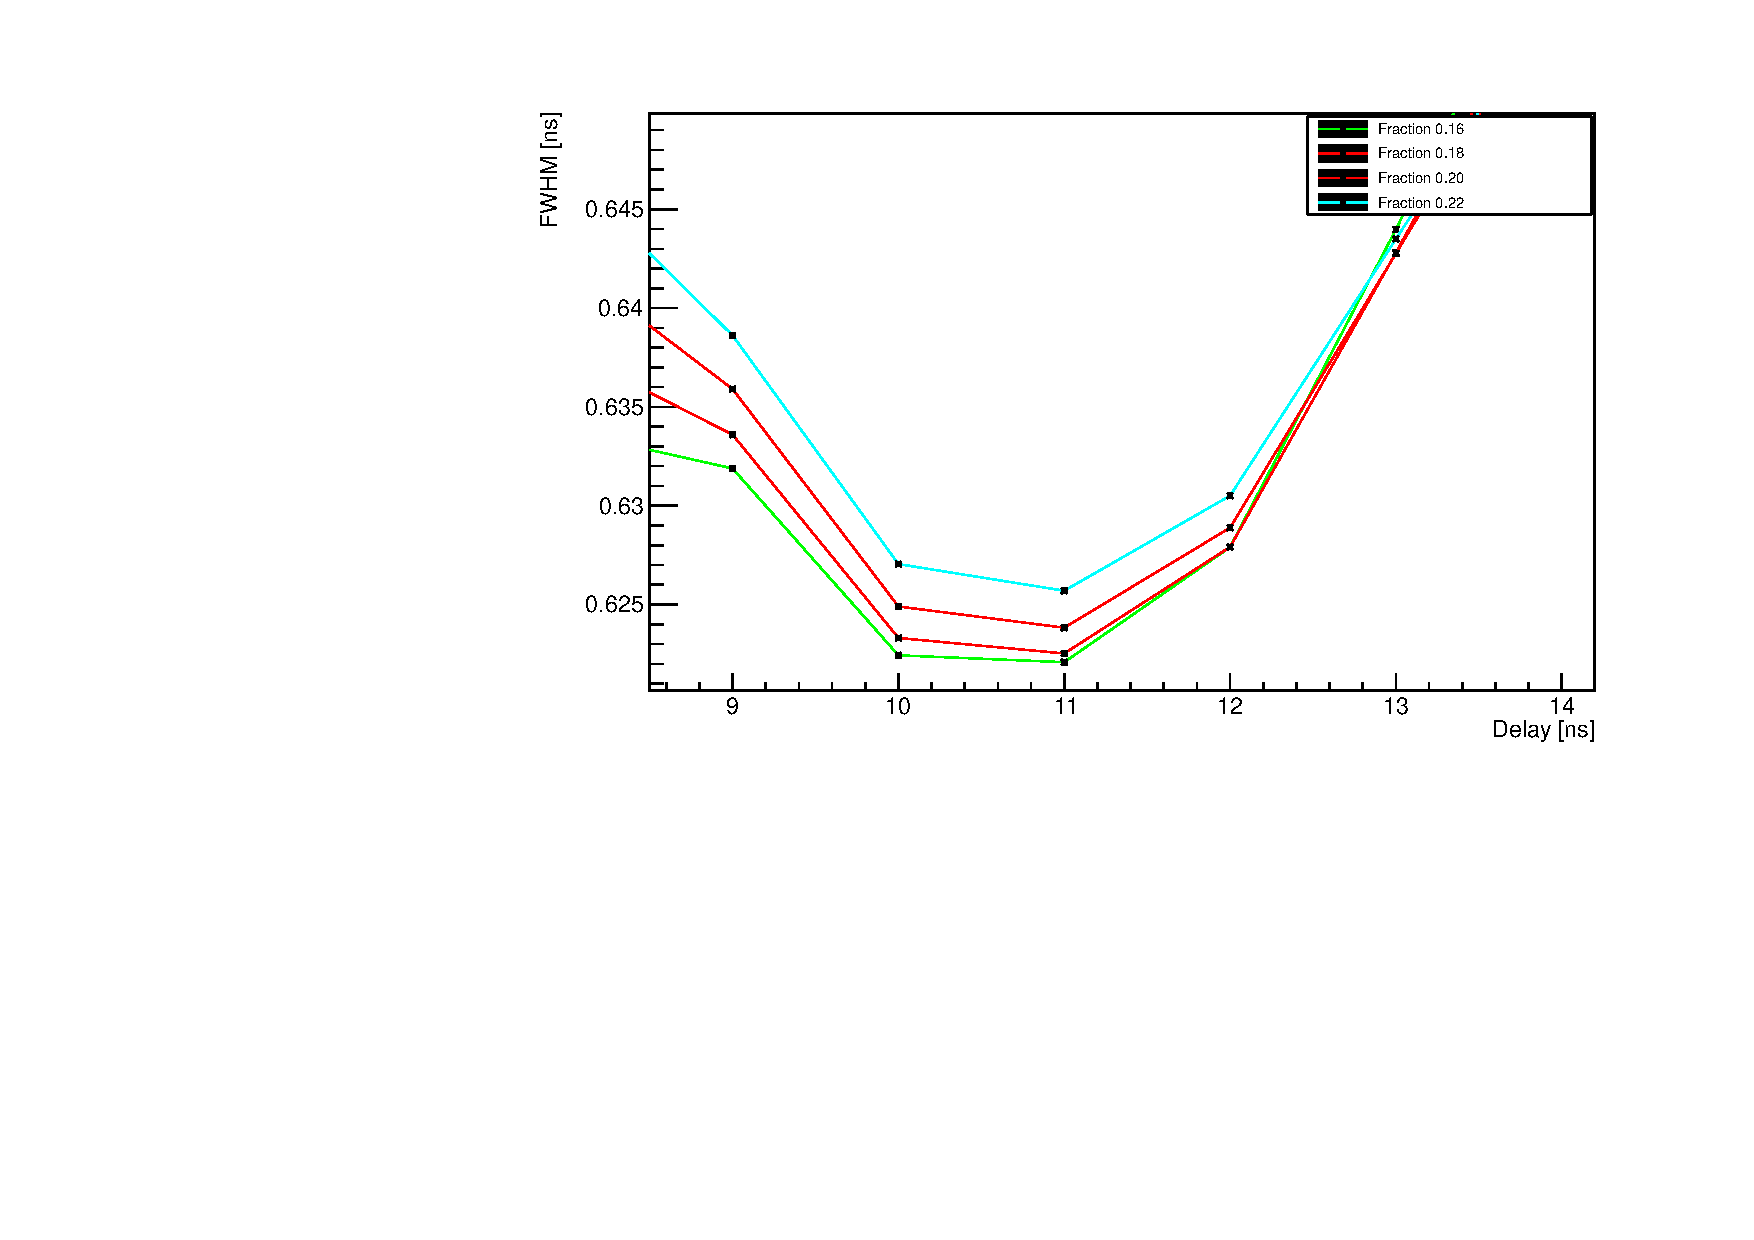
\includegraphics[width=.48\textwidth]{8_14_del}} \\
 	\caption{FWHM as a function of \emph{Fraction} (a) and \emph{Delay} (b). The different curves represent different value of the second parameter.}
 	\label{Fig:fd_opt}
 \end{figure}
 
 Using the selected fraction/delay configuration, the best zero crossing line value is computed in order to minimize the time walk. Fig.~\ref{Fig:Zcl} shows the FHWM of timing distributions obtained from the whole energy spectrum from different zero crossing line values.  
 
\begin{figure}[H]
	\centering
 	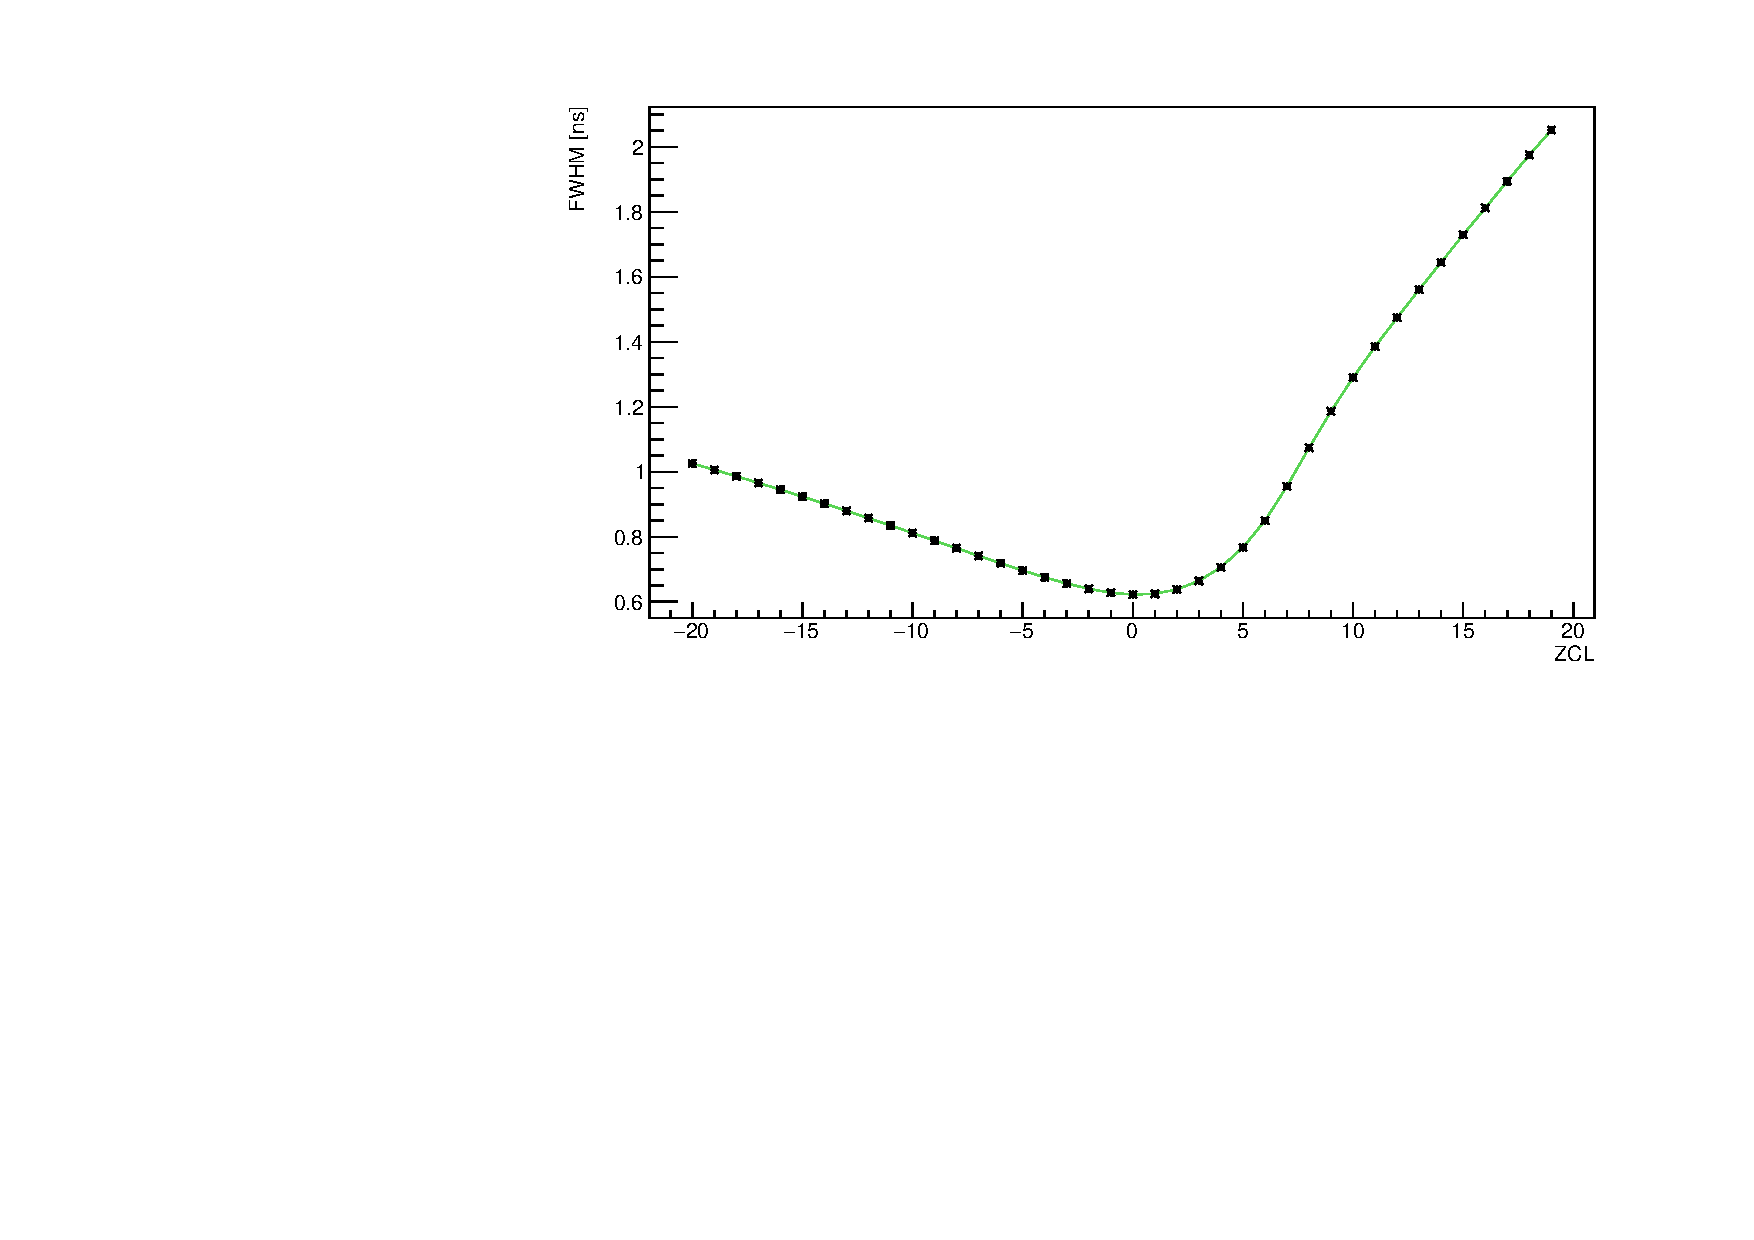
\includegraphics[width=\textwidth]{ZCL_opt}
 	\caption{FWHM as a function of zero crossing line.}
 	\label{Fig:Zcl}
 \end{figure}
 
 Finally, with the optimized parameters, was possible to perform the digital timing analysis. The $^{22}$Na source was used, similarly to the analog timing the FWHM of distributions obtained selecting events inside energy windows of 50~keV width were computed.  Fig.~\ref{Fig:Digi2d} and Fig.~\ref{Fig:DigiDist} show respectively the distribution and the calculated FWHM for each energy windows.
 
  \begin{figure}[H]
  	\centering
  	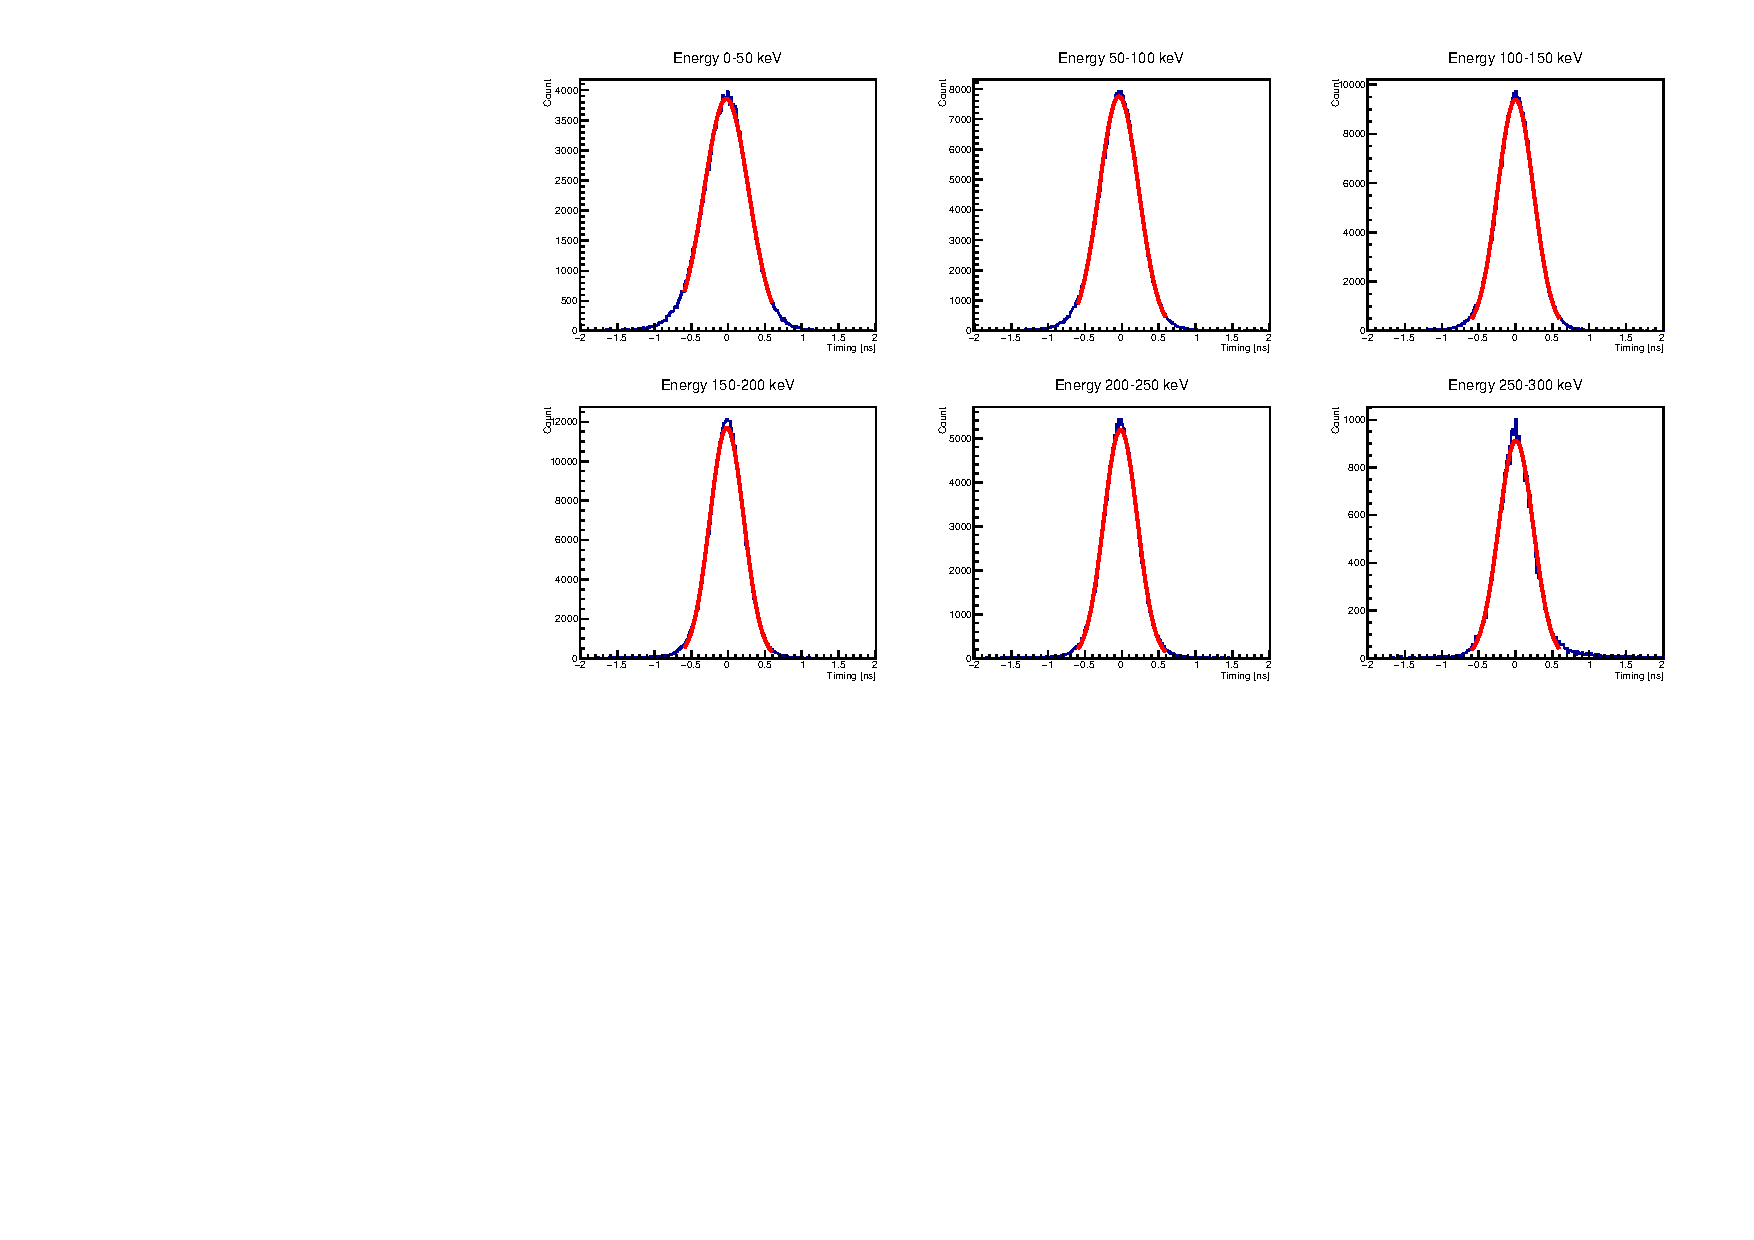
\includegraphics[width=\textwidth]{dist}
  	\caption{Digital timing distributions obtained selecting events inside 50~keV energy windows}
  	\label{Fig:DigiDist}
  \end{figure}
  
   \begin{figure}[H]
   	\centering
   	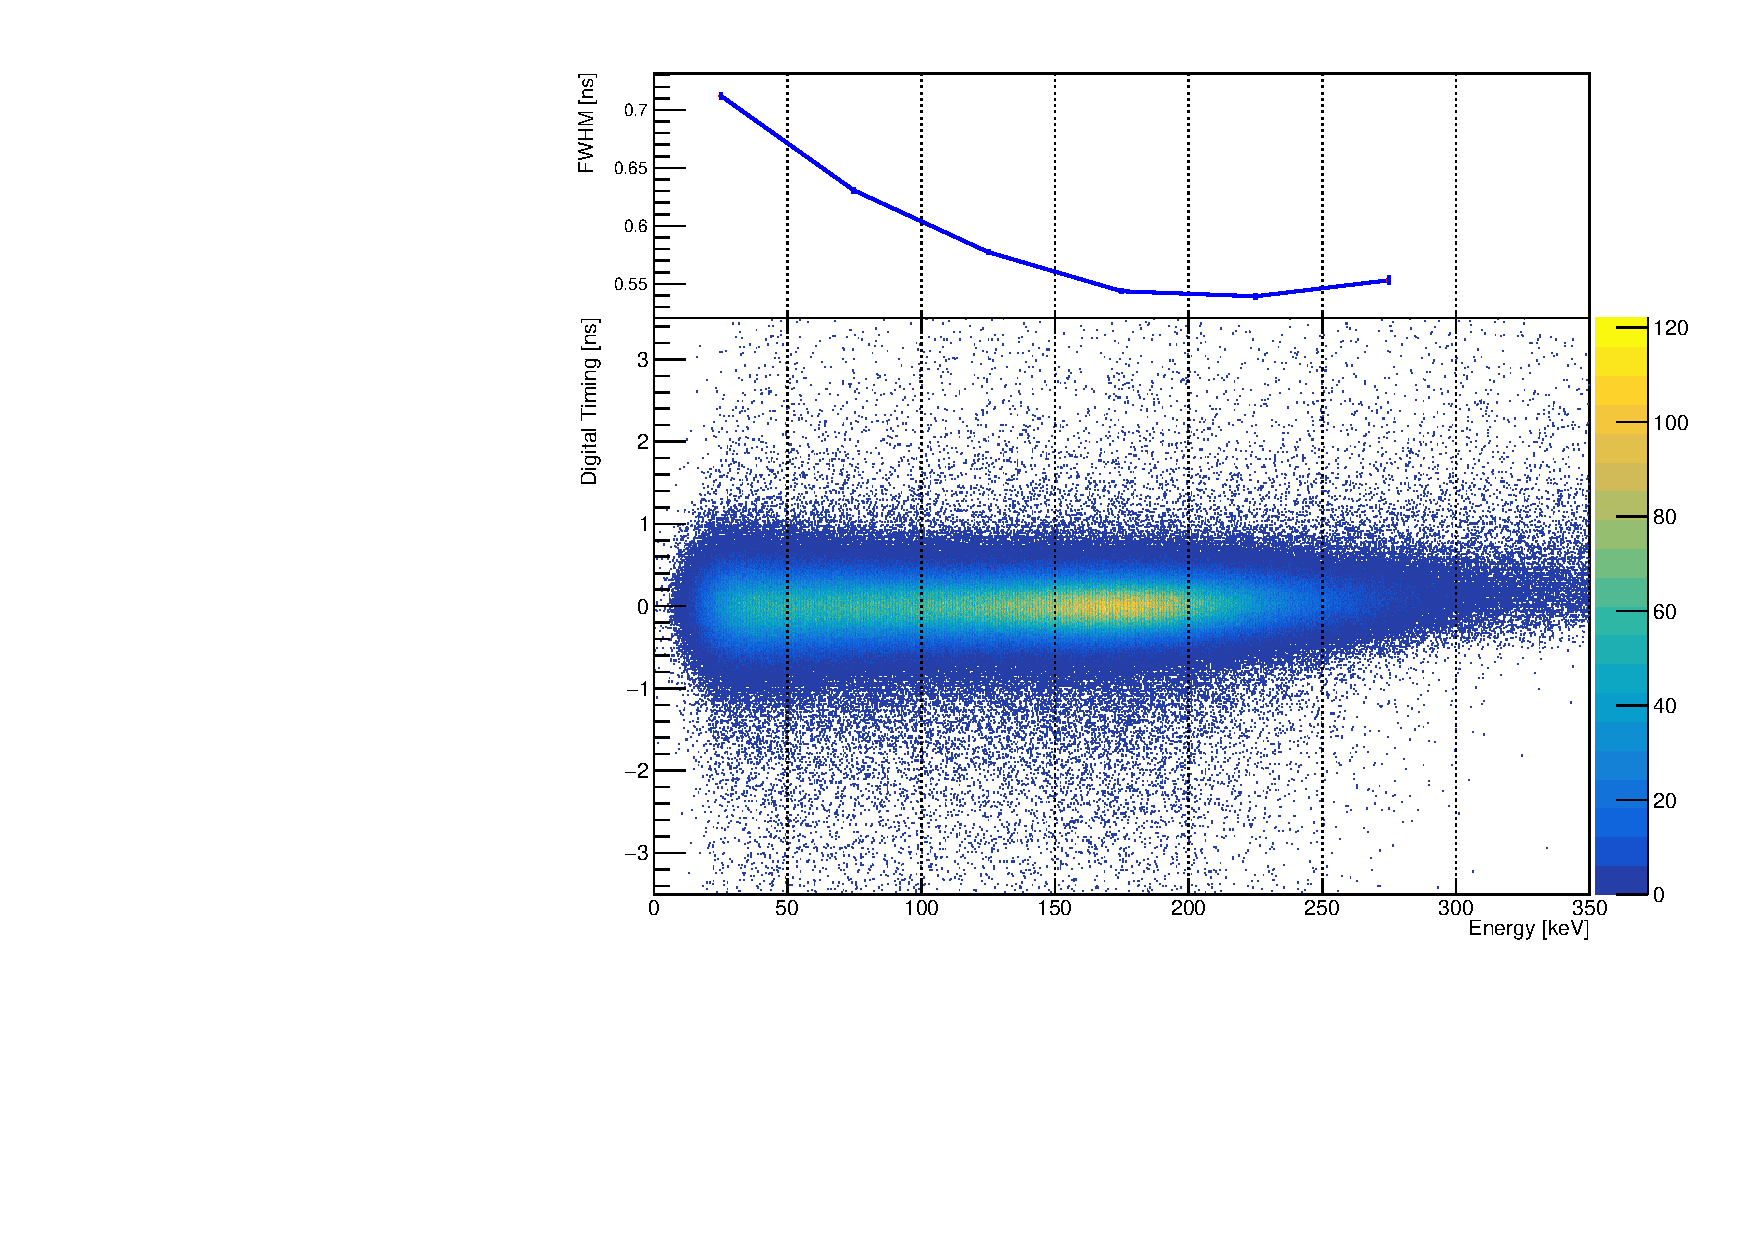
\includegraphics[width=\textwidth]{digi_timing}
   	\caption{FWHM for each energy slice over 2-D density plot of digital timing as function of energy.}
   	\label{Fig:Digi2d}
   \end{figure}